\documentclass[english]{article}
\usepackage[english]{babel} 
\usepackage[T1]{fontenc}
\usepackage[utf8x]{inputenc}
\usepackage{float}
\usepackage{graphicx}

\makeatletter
\usepackage[a4paper,top=2cm,bottom=2cm,left=2cm,right=2cm]{geometry}
\usepackage{enumitem}
\usepackage{subfig}
\usepackage{amsthm}
\usepackage{amsmath}
\usepackage{epstopdf}
\usepackage{fancyhdr}
\usepackage{booktabs,array}

\hyphenation{english}
\makeatother

\usepackage{babel}


\usepackage{listings}
\usepackage{xcolor} % for setting colors

% set the default code style
\lstset{
    frame=tb, % draw a frame at the top and bottom of the code block
    tabsize=4, % tab space width
    showstringspaces=false, % don't mark spaces in strings
    numbers=left, % display line numbers on the left
    commentstyle=\color{gray}, % comment color
    keywordstyle=\color{blue}, % keyword color
    stringstyle=\color{red} % string color
}


\begin{document}
\begin{titlepage}

	\begin{center}
		\begin{Large} \textbf{UNIVERSITY OF PADOVA} \\
		\end{Large} \vspace{1cm}
		\vspace{3cm}
		\begin{Large} Embedded Real--Time Control \end{Large}
		\par\end{center}

	\begin{center}
		\begin{Large}Laboratory report\\
		\end{Large}
		\par\end{center}

	\begin{center}
		\vspace{2cm}
		\begin{figure}[!htb]
			\centering \includegraphics[width=8cm]{figures/unipd-logo.png}\\

		\end{figure}

		\par\end{center}

	\begin{center}
		\vspace{2cm}
		{\Large \textbf{Names} -- \textbf{Student ID Numbers}} \\[1em]

		\begin{tabular}{lc}
			Diego Marchini   & 2239741 \\
			Alessio Modonesi & 2101846 \\
			Susanna Sandoyan & 2222159 \\
			Mattia Zanini    & 2239257
		\end{tabular}

		\vspace{2cm}
		{\Large Academic Year 2026-2027}
	\end{center}

\end{titlepage}

\tableofcontents
\newpage

\section{Laboratory 1}

In this lab we learnt to interact with external devices connected to the microcontroller through serial bus communication. In particular we used I2C communication to retrieve data from a keypad peripheral and a line sensor.

\subsection{Relevant theoretical notions}

\subsubsection{I2C protocol}

\subsubsection{SX1509 I/O expander}

\subsubsection{Pololu QTR reflectance sensor}

\subsubsection{4$\times$4 keypad}

\subsubsection{Timer interrupt frequency}

\begin{figure}[!h]
	\centering
	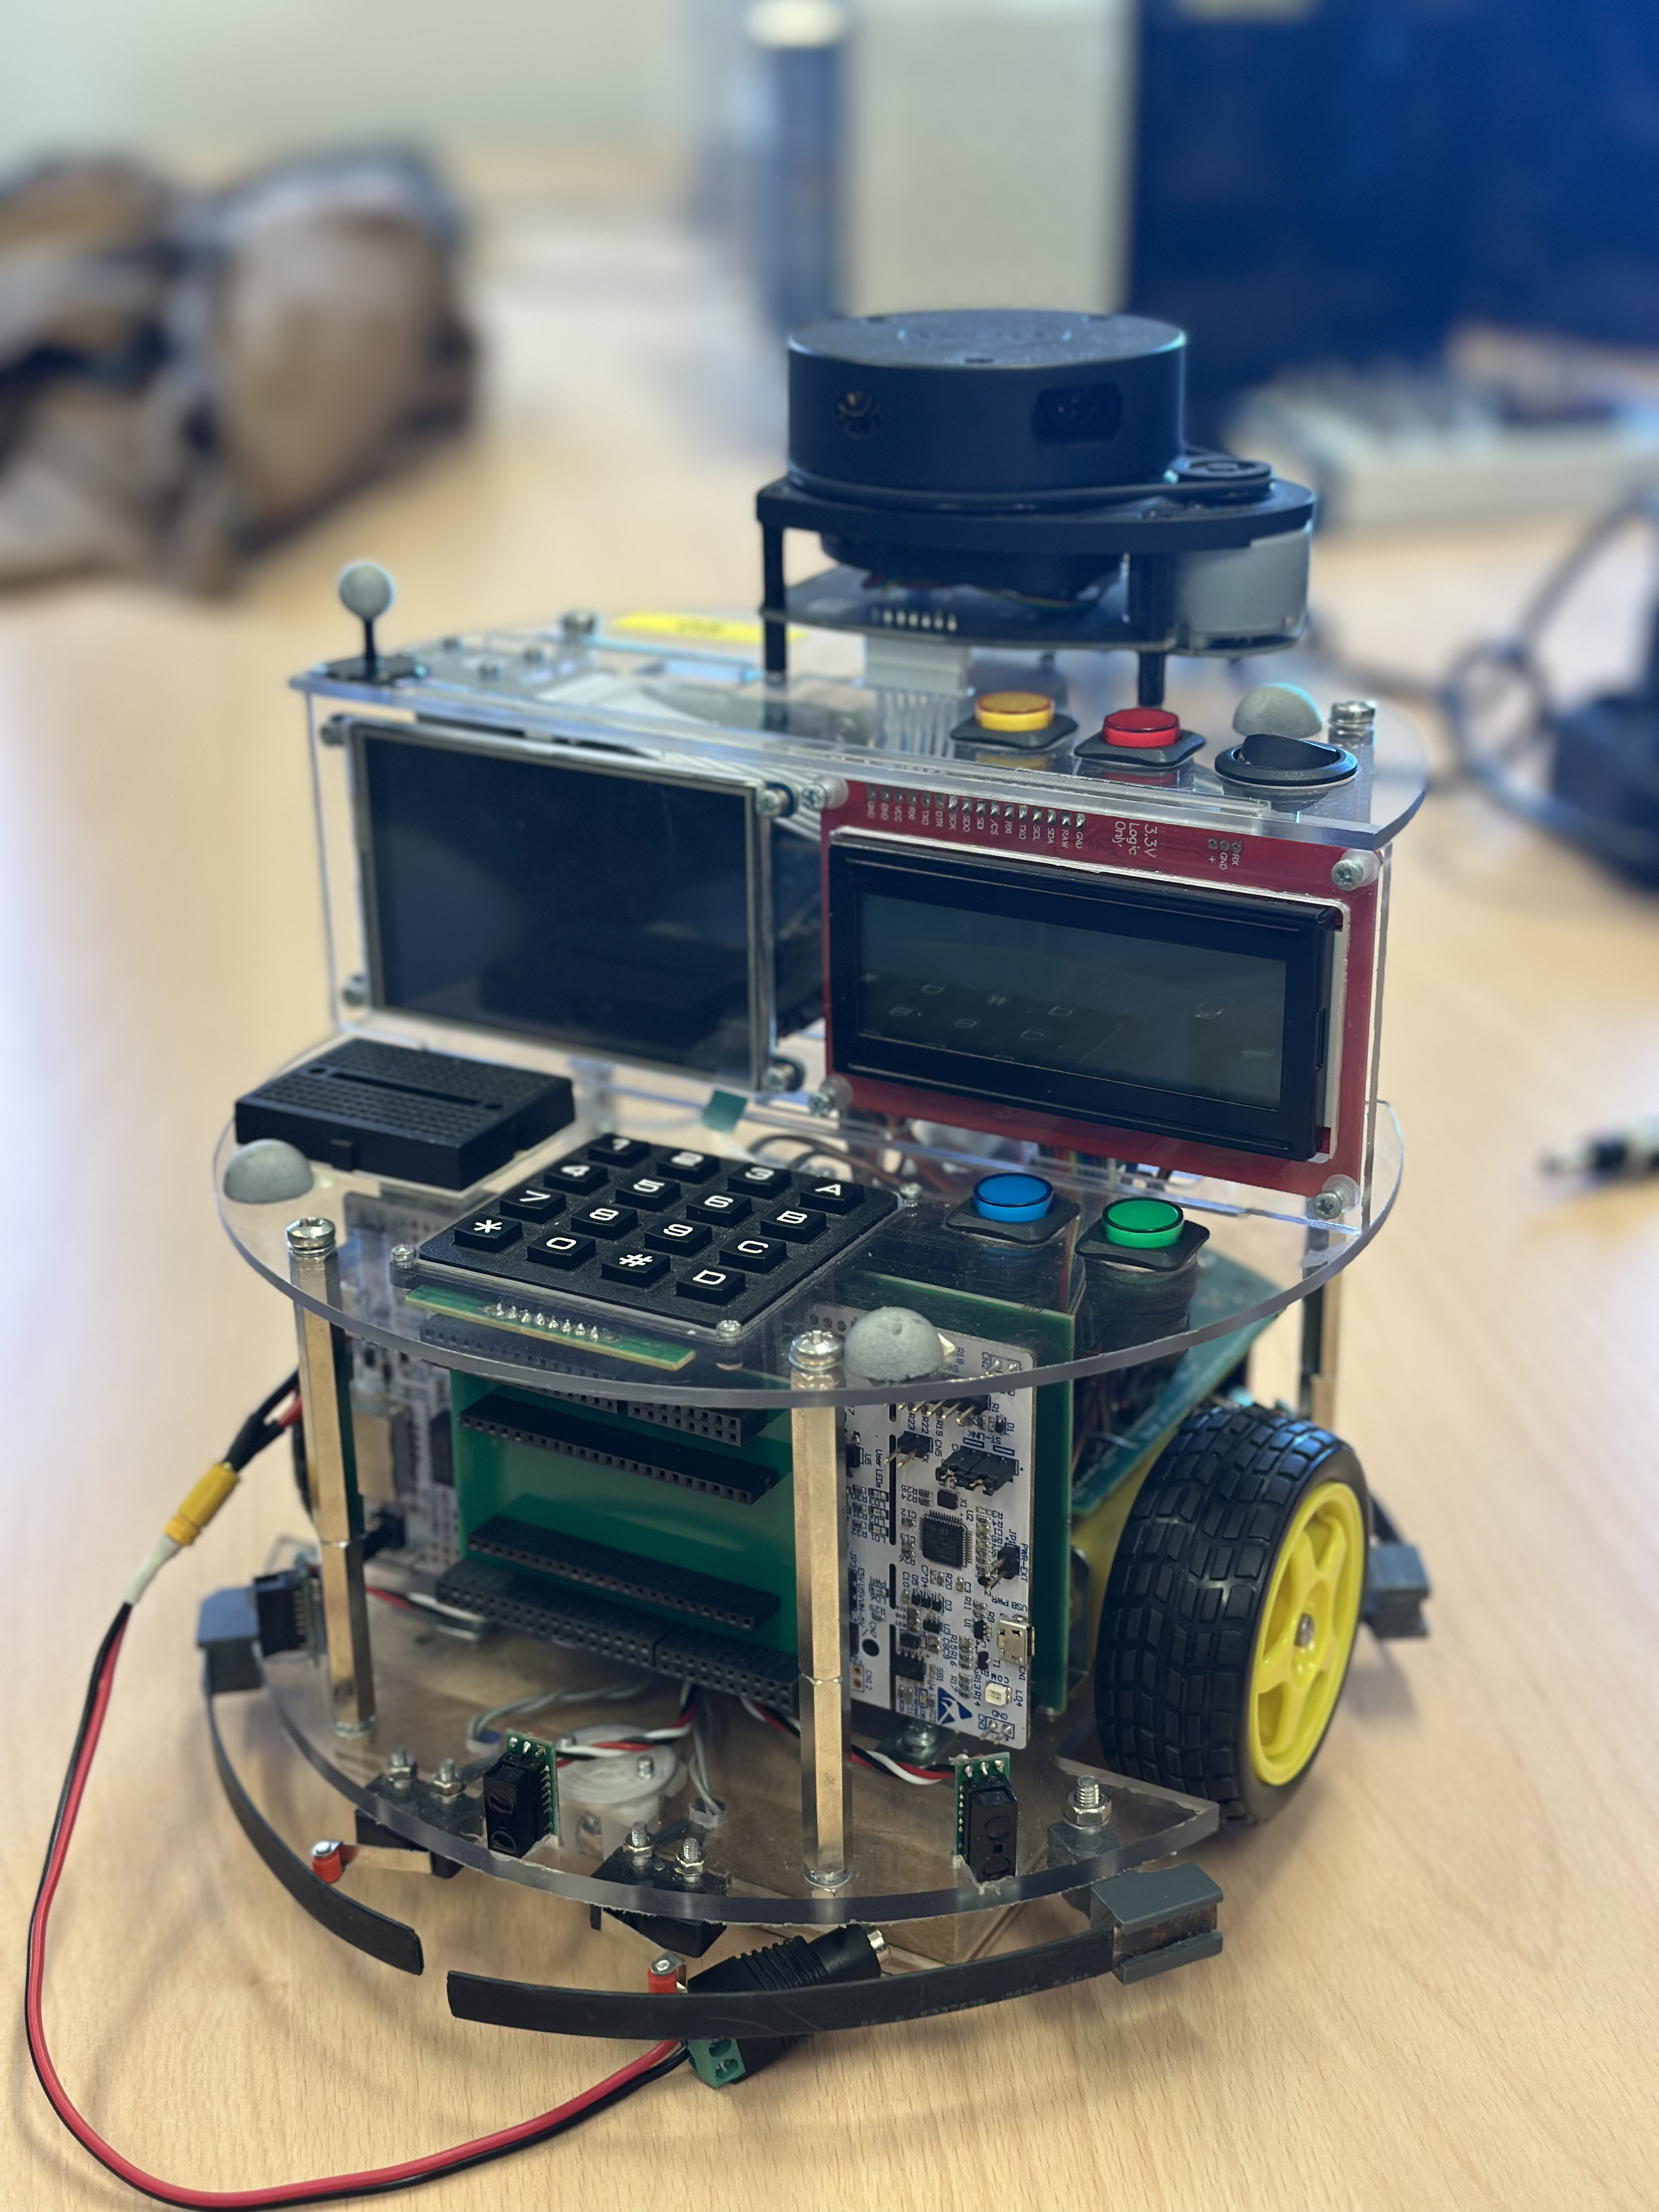
\includegraphics[width=0.4\textwidth]{figures/turtlebot_1.jpg}
	\caption{The TurtleBot}
	\label{fig:turtlebot}
\end{figure}

In Figure~\ref{fig:turtlebot} ...

\begin{figure}[!ht]
	\centering
	\subfloat[The TurtleBot 1 ]
	{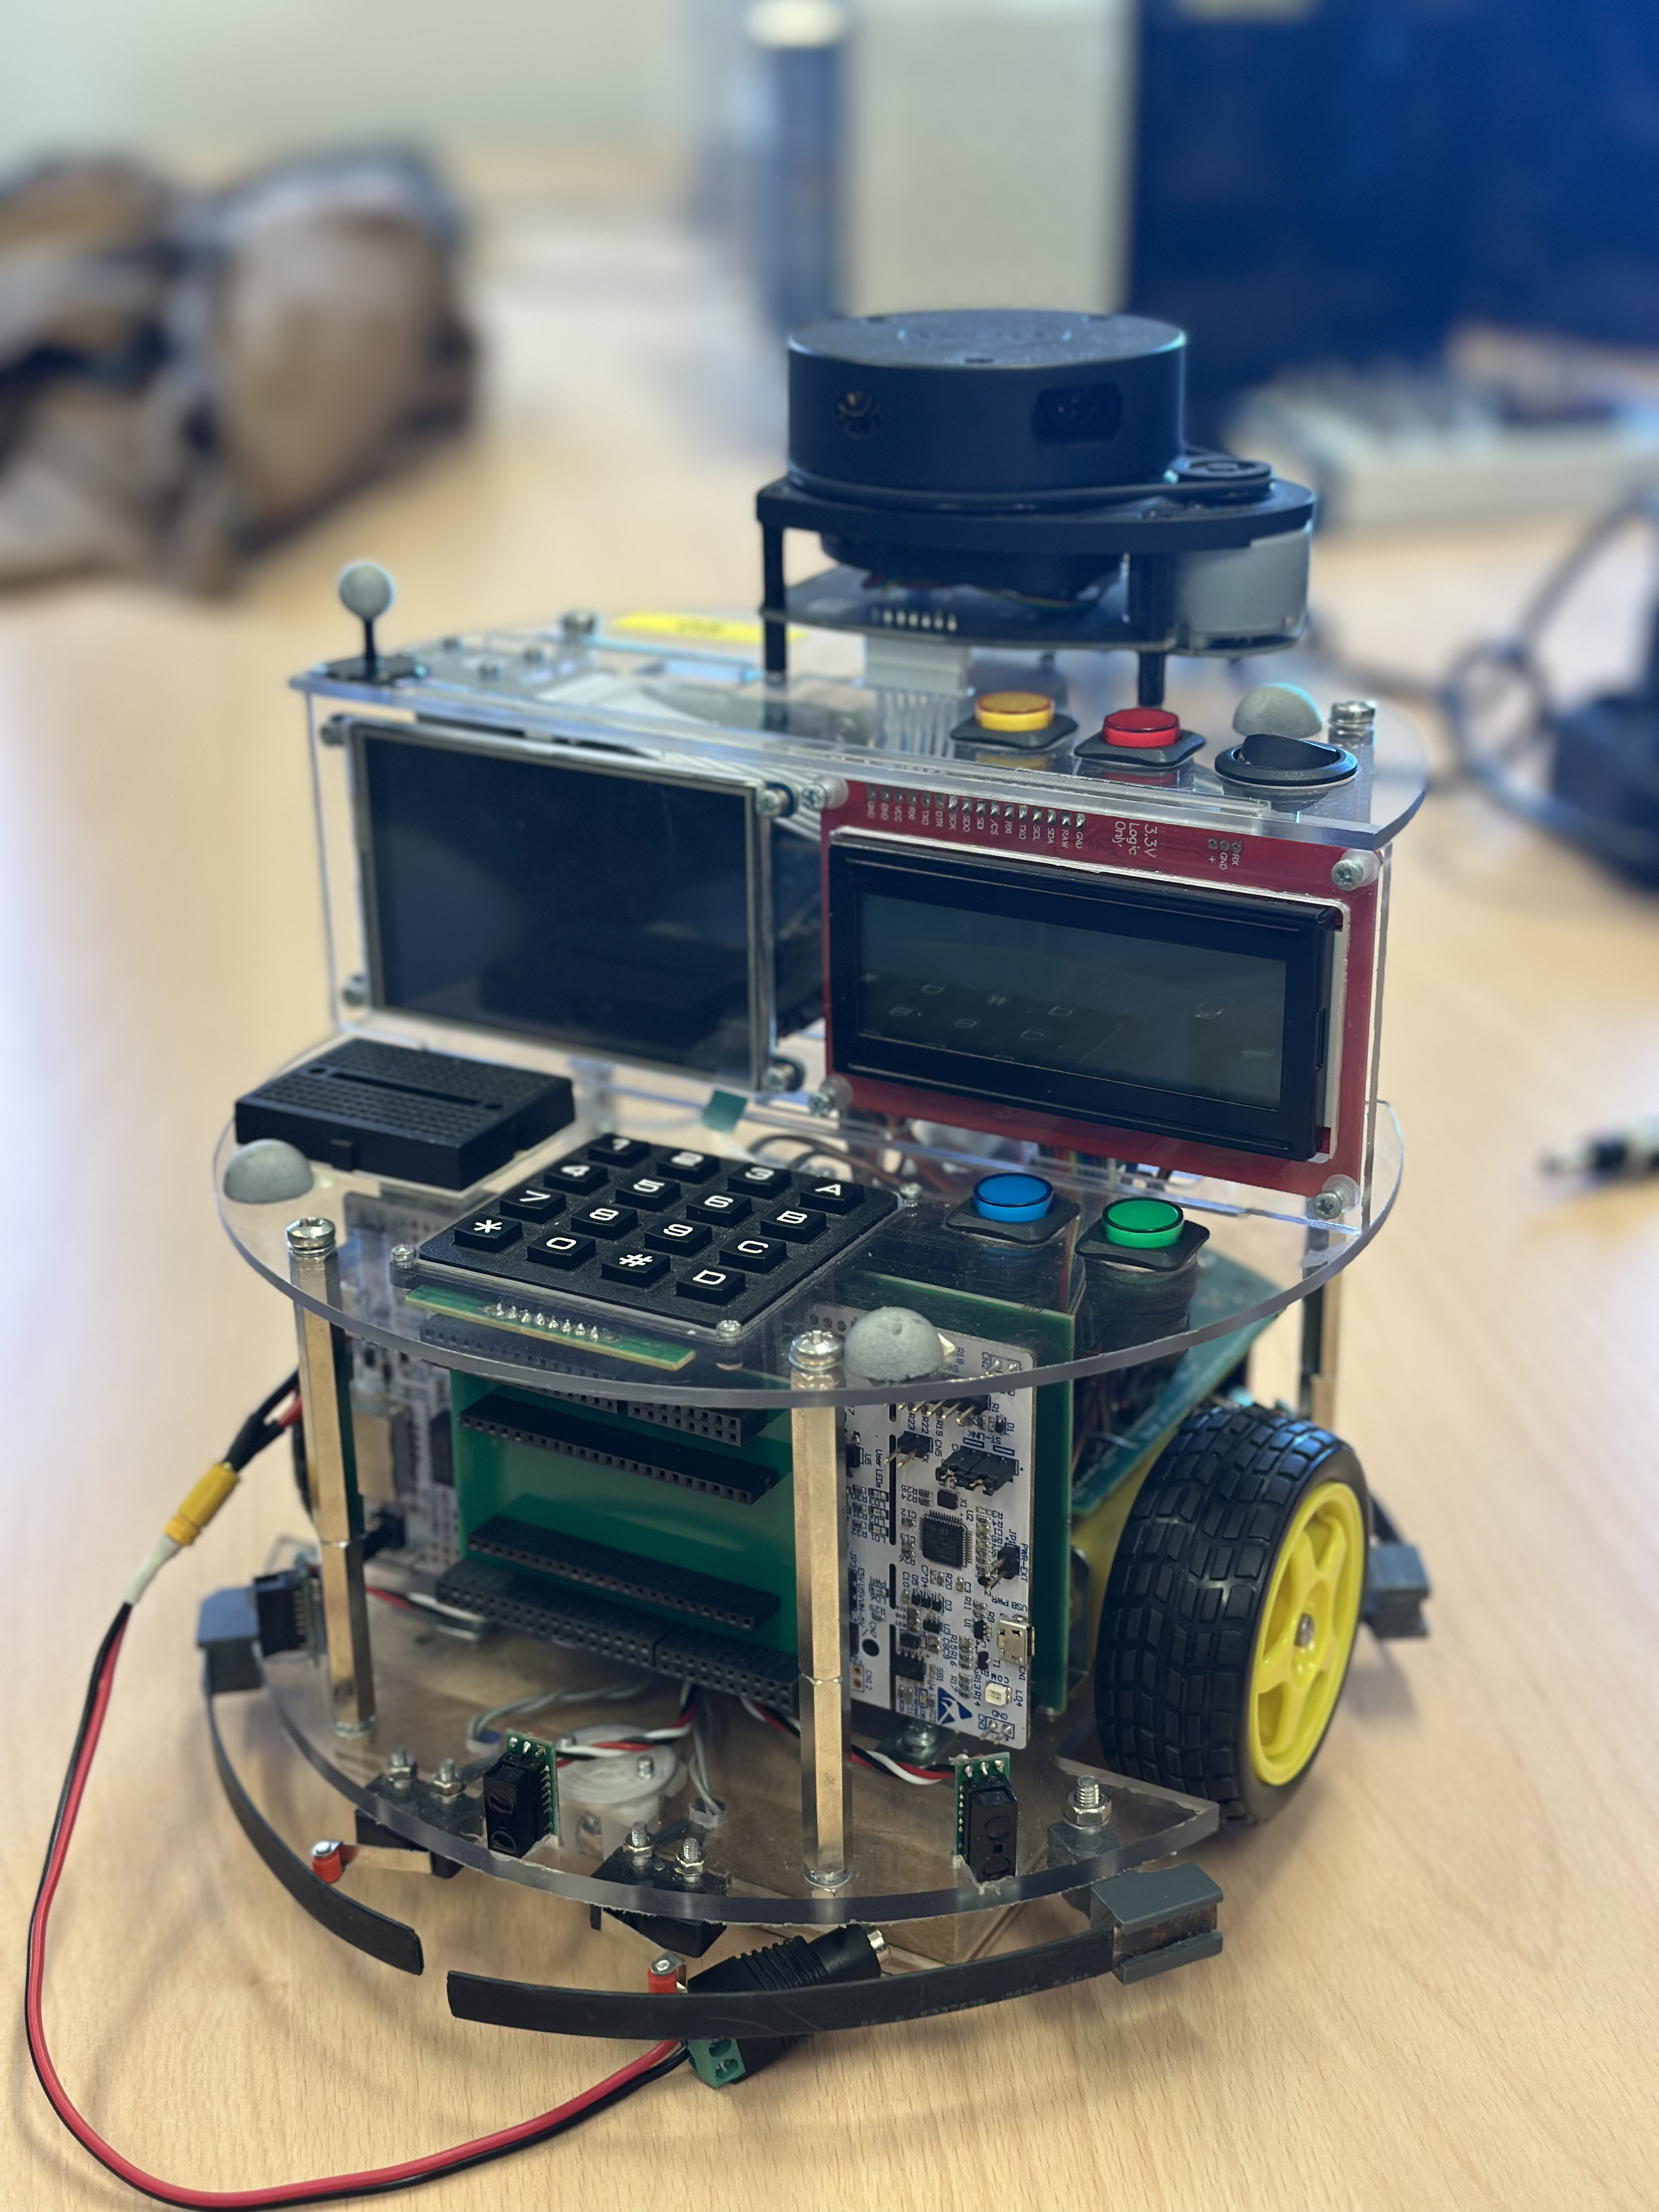
\includegraphics[width=0.3\textwidth,height=0.45\textwidth]{figures/turtlebot_1.jpg}
		\label{fig:tbot1}}
	\subfloat[The TurtleBot 2]
	{\includegraphics[width=0.3\textwidth,height=0.5\textwidth]{figures/turtlebot_2.jpg}
		\label{fig:tbot2}}
	\caption{The TurtleBot}
\end{figure}

\subsection{Brief Introduction and Objectives}

The goal of this laboratory was to execute tasks that require to access data registered by two devices: a keypad and a line sensor.
\\Each device was connected to an SX1509 general-purpose I/O expander, which was then connected to the microcontroller through I2C bus.
\\Both SX1509 devices shared the same I2C line ("i2c1") so we assigned them different slave addresses: 0x3E for "sx1509\_1" (line sensor) and 0x3F for "sx1509\_2" (keypad). 
\\The laborarory was split into five exercises of increasing complexity: handling the keypad interrupt (Ex. 1), decoding the pressed key (Ex. 2), polling the line sensor by sotware (Ex. 3), polling the line sensor via timer interrupt (Ex. 4), and using the keypad to set the blinking frequency of an LED (Ex. 5, with "easy" and "hard" variants).

\subsection{Problem Analysis}


\subsection{Theoretical Background}
Describe the relevant theoretical concepts, mathematical models, equations, or physical laws applied.

For example, considering a continuous transfer function:
\begin{equation}
	G(s) = \frac{K}{\tau s + 1} e^{-\theta s}
\end{equation}
Explain how this theoretical baseline guides the implementation choice or controller structure.

\subsection{Design \& Implementation Choices}

Detail your design decisions, thought process, and engineering trade-offs.

\subsubsection{Tools \& Software Environment}

\begin{itemize}
	\item \textbf{MATLAB / Simulink:} Used for offline parameter identification and simulation.
	\item \textbf{C / C++ / Embedded IDE:} Used for real-time firmware execution.
\end{itemize}

\subsubsection{Code Structure}

\begin{lstlisting}[language=C, caption={C code using listings}, label={lst:label} ]
#include <stdio.h>
int main()
{
	// print hello to the console
	printf("Hello, world!");
	return 0;
}
\end{lstlisting}

See code~\ref{lst:label}.

\subsection{Controller Design (If Applicable)}

If the activity involved control system synthesis:
\begin{itemize}
	\item State desired requirements (e.g., Settling Time $T_s < 1.0\,\text{s}$, Phase Margin $\phi_m > 45^\circ$).
	\item Detail the tuning method (e.g., pole placement, root locus, frequency response tuning).
\end{itemize}

\subsection{Discovered Issues, Calibration \& Workarounds}

This section captures critical unexpected findings during execution:
\begin{itemize}
	\item \textbf{Unforeseen Issues:} Detail any problems not noticed during the design phase (e.g., noise on sensor pins, numerical overflow).
	\item \textbf{Calibration \& Performance Gaps:} If the controller did not achieve perfect calibration or desired performance, explain why (e.g., unmodeled dynamics, saturation limits, transport delay) and propose plausible fixes.
	\item \textbf{Original / Experimental Solutions:} If original or non-standard approaches were tried, describe why they were developed and assess their success or failure.
\end{itemize}

\subsection{Results and Graphical Analysis}

Present collected measurements, plots, and experimental data. Describe what each plot demonstrates rather than just attaching graphics.

\begin{figure}[htbp]
	\centering
	\framebox[0.85\textwidth]{\vbox to 45mm{\vfill \centerline{\textit{[ Insert Step Response Plot / Data Visualisation Here ]}} \vfill}}
	\caption{Step response comparison: Target trajectories vs. Measured output.}
	\label{fig:step_response}
\end{figure}

\subsection{Conclusions}

Summarise the key learnings, whether the initial objectives were reached, and what improvements could be introduced in future iterations.

\clearpage
\appendix

\section{Section in the Appendix}
\label{sec:app1}

\subsection{Subsection in the Appendix}
\label{subsec:app2}

Additional relevant information...

\end{document}